
%%%%%%%%%%%%%%%%%%%%%%%%%%%%%%%%%%%%%%%%%
% Beamer Presentation
% LaTeX Template
% Version 1.0 (10/11/12)
%
% This template has been downloaded from:
% http://www.LaTeXTemplates.com
%
% License:
% CC BY-NC-SA 3.0 (http://creativecommons.org/licenses/by-nc-sa/3.0/)
%
%%%%%%%%%%%%%%%%%%%%%%%%%%%%%%%%%%%%%%%%%

%----------------------------------------------------------------------------------------
%	PACKAGES AND THEMES
%----------------------------------------------------------------------------------------

\documentclass{beamer}


\usepackage{graphicx} % Allows including images
\usepackage{booktabs} % Allows the use of \toprule, \midrule and \bottomrule in tables
\usepackage[brazil]{babel}
\usepackage[utf8]{inputenc}
\usepackage{caption}  %Allows including capitons on images
%\usepackage{subcaption} %allow including multiples figures side to side
\usepackage{ragged2e} %allows justify text in tables
\usepackage{ulem} %allows striker text
\usepackage{subfigure}
\usepackage{hyperref}
\usepackage{color}
\usepackage{ragged2e}
\usepackage{listings}
\usepackage[3D]{movie15}

\mode<presentation> {

% The Beamer class comes with a number of default slide themes
% which change the colors and layouts of slides. Below this is a list
% of all the themes, uncomment each in turn to see what they look like.

%\usetheme{default}
%\usetheme{AnnArbor}
%\usetheme{Antibes}
%\usetheme{Bergen}
%\usetheme{Berkeley}
%\usetheme{Berlin}
%\usetheme{Boadilla}
%\usetheme{CambridgeUS}
%\usetheme{Copenhagen}
\usetheme{Darmstadt}
%\usetheme{Dresden}
%\usetheme{Frankfurt}
%\usetheme{Goettingen}
%\usetheme{Hannover}
%\usetheme{Ilmenau}
%\usetheme{JuanLesPins}
%\usetheme{Luebeck}
%\usetheme{Madrid}
%\usetheme{Malmoe}
%\usetheme{Marburg}
%\usetheme{Montpellier}
%\usetheme{PaloAlto}
%\usetheme{Pittsburgh}
%\usetheme{Rochester}
%\usetheme{Singapore}
%\usetheme{Szeged}
%\usetheme{Warsaw}

% As well as themes, the Beamer class has a number of color themes
% for any slide theme. Uncomment each of these in turn to see how it
% changes the colors of your current slide theme.

%\usecolortheme{albatross}
%\usecolortheme{beaver}
%\usecolortheme{beetle}
%\usecolortheme{crane}
%\usecolortheme{dolphin}
%\usecolortheme{dove}
%\usecolortheme{fly}
%\usecolortheme{lily}
%\usecolortheme{orchid}
\usecolortheme{rose}
%\usecolortheme{seagull}
%\usecolortheme{seahorse}
%\usecolortheme{whale}
%\usecolortheme{wolverine}


% Set Font

%\usefonttheme{default}
%\usefonttheme{professionalfonts}
%\usefonttheme{serif}
%\usefonttheme{structurebold}
%\usefonttheme{structureitalicserif}

%\setbeamertemplate{footline} % To remove the footer line in all slides uncomment this line
%\setbeamertemplate{footline}[page number] % To replace the footer line in all slides with a simple slide count uncomment this line

%\setbeamertemplate{navigation symbols}{} % To remove the navigation symbols from the bottom of all slides uncomment this line

}



\definecolor{mygreen}{rgb}{0,0.6,0}
\definecolor{mygray}{rgb}{0.5,0.5,0.5}
\definecolor{mymauve}{rgb}{0.58,0,0.82}

\lstset{ %
  backgroundcolor=\color[rgb]{0.98, 1, 0.75},   % choose the background color; you must add \usepackage{color} or \usepackage{xcolor}
  basicstyle=\ttfamily\scriptsize,        % the size of the fonts that are used for the code
  breakatwhitespace=false,         % sets if automatic breaks should only happen at whitespace
  breaklines=true,                 % sets automatic line breaking
  captionpos=b,                    % sets the caption-position to bottom
  commentstyle=\color{mygreen},    % comment style
  deletekeywords={...},            % if you want to delete keywords from the given language
  escapeinside={\%*}{*)},          % if you want to add LaTeX within your code
  extendedchars=true,              % lets you use non-ASCII characters; for 8-bits encodings only, does not work with UTF-8
  frame=single,                    % adds a frame around the code
  keepspaces=true,                 % keeps spaces in text, useful for keeping indentation of code (possibly needs columns=flexible)
  keywordstyle=\color{blue},       % keyword style
  language=Java,                 % the language of the code
  morekeywords={*,...},            % if you want to add more keywords to the set
  numbers=left,                    % where to put the line-numbers; possible values are (none, left, right)
  numbersep=5pt,                   % how far the line-numbers are from the code
  numberstyle=\tiny\color{mygray}, % the style that is used for the line-numbers
  rulecolor=\color{black},         % if not set, the frame-color may be changed on line-breaks within not-black text (e.g. comments (green here))
  showspaces=false,                % show spaces everywhere adding particular underscores; it overrides 'showstringspaces'
  showstringspaces=false,          % underline spaces within strings only
  showtabs=false,                  % show tabs within strings adding particular underscores
  stepnumber=2,                    % the step between two line-numbers. If it's 1, each line will be numbered
  stringstyle=\color{mymauve},     % string literal style
  tabsize=2,                       % sets default tabsize to 2 spaces
  title=\lstname                   % show the filename of files included with \lstinputlisting; also try caption instead of title
}

%----------------------------------------------------------------------------------------
%	VIDEO CONFIG
%----------------------------------------------------------------------------------------




%----------------------------------------------------------------------------------------
%	TITLE PAGE
%----------------------------------------------------------------------------------------

\title[Simuladores aula 2]{Simuladores aula 2} % The short title appears at the bottom of every slide, the full title is only on the title page

\author{Bruno Pereira} % Your name
\institute[UFMG] % Your institution as it will appear on the bottom of every slide, may be shorthand to save space
{
Universidade Federal de Minas Gerais \\ % Your institution for the title page
\medskip
\textit{bruno.ps@dcc.ufmg.com} % Your email address
}
\date{\tiny\today} % Date, can be changed to a custom date

\begin{document}


\begin{frame}
\titlepage % Print the title page as the first slide
\end{frame}

\begin{frame}
\frametitle{Agenda} % Table of contents slide, comment this block out to remove it
\tableofcontents % Throughout your presentation, if you choose to use \section{} and \subsection{} commands, these will automatically be printed on this slide as an overview of your presentation
\end{frame}

%----------------------------------------------------------------------------------------
%	PRESENTATION SLIDES
%----------------------------------------------------------------------------------------

%------------------------------------------------
\section{Continuando...} % Sections can be created in order to organize your presentation into discrete blocks, all sections and subsections are automatically printed in the table of contents as an overview of the talk
%------------------------------------------------

\subsection{Aula passada} % A subsection can be created just before a set of slides with a common theme to further break down your presentation into chunks
%------------------------------------------------

\begin{frame}\frametitle{Exercício PingPong}

	\begin{block}{Conceitos}
		\begin{enumerate}
			\item Comportamento do nó
			\item Modelos
			\item Criar um arquivo de configuração
		\end{enumerate}
	\end{block}

	\begin{exampleblock}{Comportamento PingPong}<2->
	\begin{itemize}
		\item Nesta simulação, dois nós vão trocar mensagens entre si.
		\item Os nós geram cores em RGB de modo aleatório.
		\item Cada cor gerada deve ser anexada em uma mensagem, que será enviada para o vizinho.
		\item Ao receber uma mensagem:
		\begin{itemize}
			\item O nó deve alterar sua cor conforme os valores RBG recebidos.
			\item Gerar uma nova cor RGB e enviar por broadcast.
		\end{itemize}
	\end{itemize}
	\end{exampleblock}

\end{frame}
%------------------------------------------------

\begin{frame}\frametitle{Exercícios da aula passada}

	\begin{exampleblock}{Ping Pong}
		\begin{figure}[t]
			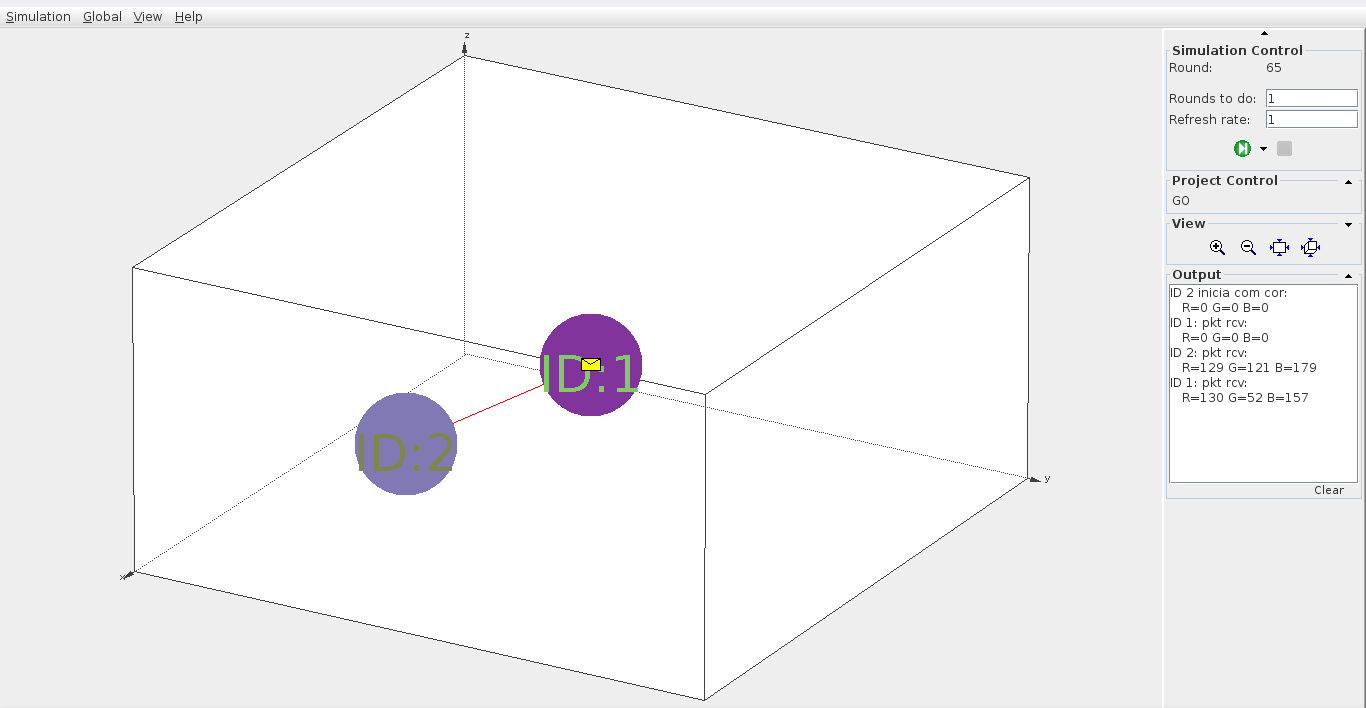
\includegraphics[width=1\linewidth]{img/pingpong.png}
		\end{figure}
	\end{exampleblock}
\end{frame}
%------------------------------------------------

\begin{frame}\frametitle{Exercícios da aula passada}
	\begin{alertblock}{Tarefa 1}
		\begin{enumerate}
			\item Execute os 6 exemplos do Sinalgo.
			\item Descreva a finalidade do exemplo.
			\item Quais conceitos visto em sala de aula que são demonstrados em cada exemplo.
			\item Descreva as limitações de cada exemplo.
			\item Quais os pontos fortes e fracos do Sinalgo?
		\end{enumerate}
	\end{alertblock}
\end{frame}


%------------------------------------------------
\section{Outros simuladores} % Sections can be created in order to organize your presentation into discrete blocks, all sections and subsections are automatically printed in the table of contents as an overview of the talk
%------------------------------------------------

\begin{frame}
    \centering
    Outros simuladores
\end{frame}

\subsection{The Network Simulator - NS2}

\begin{frame}

\begin{block}{NS2}
	\begin{itemize}
		\item Discrete event simulator
		\item Support for simulation of TCP
		\item Support routing protocols
		\item Multicast protocols over wired and wireless (local and satellite) networks
		\item \textbf{Aqua-SIM}
		\item \href{https://www.nsnam.org/}{\textcolor{red}{\textbf{NS3}}}.
	\end{itemize}
\end{block}

\end{frame}

%------------------------------------------------
\begin{frame}

\begin{exampleblock}{Vídeo}
	\centering
    \includemovie[autoplay,controls]{1\linewidth}{.65\linewidth}{video/NetworkSimulation(UDPTCP).mp4}
\end{exampleblock}

\end{frame}


%------------------------------------------------
\subsection{OMNeT++}

\begin{frame}

\begin{exampleblock}{Vídeo}<2->
	\centering
	\includemovie[autoplay,controls]{1\linewidth}{.375\linewidth}{video/OMNeT++Demo.mp4}
\end{exampleblock}

\begin{block}{OMNeT++}

\begin{columns}[c] % The "c" option specifies centered vertical alignment while the "t" option is used for top vertical alignment

\column{.5\textwidth} % Left column and width
	\begin{itemize}
		\item Component-based C++
		\item Support for sensor networks
	\end{itemize}
\column{.5\textwidth} % Left column and width
\begin{itemize}
		\item Wireless ad-hoc networks
		\item Internet protocols
	\end{itemize}
\end{columns}
\end{block}
\end{frame}

%------------------------------------------------
\subsection{Castalia}

\begin{frame}

\begin{block}{Castalia}
Castalia is a simulator based on the OMNeT++ for WSN.
	\begin{itemize}
		\item Advanced channel model based on empirically measured data
		\item Advanced radio model based on real radios for low-power communication
		\item Extended sensing modelling provisions
		\item MAC and routing protocols available
		\item \textit{Body Area Networks (BAN)}
	\end{itemize}
\end{block}
\end{frame}

%------------------------------------------------
\subsection{SUMO}

\begin{frame}

\begin{block}{Sumo -- Simulation of Urban MObility}

	\begin{itemize}
		\item Microscopic simulation - vehicles, pedestrians and public transport are modeled explicitly
		\item Online interaction – control the simulation with TraCI
		\item Simulation of multimodal traffic, e.g., vehicles, public transport and pedestrians
		\item Time schedules of traffic lights can be imported or generated automatically by SUMO
		\item No artificial limitations in network size and number of simulated vehicles
		\item Supported import formats: OpenStreetMap, VISUM, VISSIM, NavTeq
		\item SUMO is implemented in C++ and uses only portable libraries
	\end{itemize}

\end{block}
\end{frame}

%------------------------------------------------
\begin{frame}

\begin{exampleblock}{Vídeo}
	\centering
	\includemovie[autoplay,controls]{1\linewidth}{.7\linewidth}{video/sumo.mp4}
\end{exampleblock}

\end{frame}
%------------------------------------------------
\subsection{The ONE}

\begin{frame}

\begin{block}{The Opportunistic Network Environment simulator}

	\begin{itemize}
		\item Generating node movement using different movement models
		\item Routing messages between nodes with various DTN routing algorithms and sender and receiver types
		\item Visualizing both mobility and message passing in real time in its GUI
		\item ONE can import mobility data from real-world traces or other mobility generators.
	\end{itemize}

\end{block}

\begin{exampleblock}{Vídeo}<2->
	\centering
	\includemovie[autoplay,controls]{1\linewidth}{.375\linewidth}{video/DTN-ONE.mp4}
\end{exampleblock}


\end{frame}


%------------------------------------------------
\subsection{TOSSIM}

\begin{frame}

\begin{block}{TOSSIM -- TinyOS}

	\begin{itemize}
		\item TOSSIM is a TinyOS library
		\item TinyOS code is the same for TOSSIM
		\item TOSSIM supports two programming interfaces: Python and C++
			\begin{itemize}
				\item Python allows you to interact with a running simulation dynamically
			\end{itemize}
	\end{itemize}

\end{block}
\end{frame}
%------------------------------------------------
\subsection{Cooja}

\begin{frame}

\begin{block}{Cooja -- Contiki}

	\begin{itemize}
		\item Cooja is the Contiki network simulator.
		\item Cooja allows large and small networks
		\item Motes can be emulated at the hardware level
	\end{itemize}

\end{block}

\begin{block}{Cooja -- Contiki}

	\begin{figure}[t]
		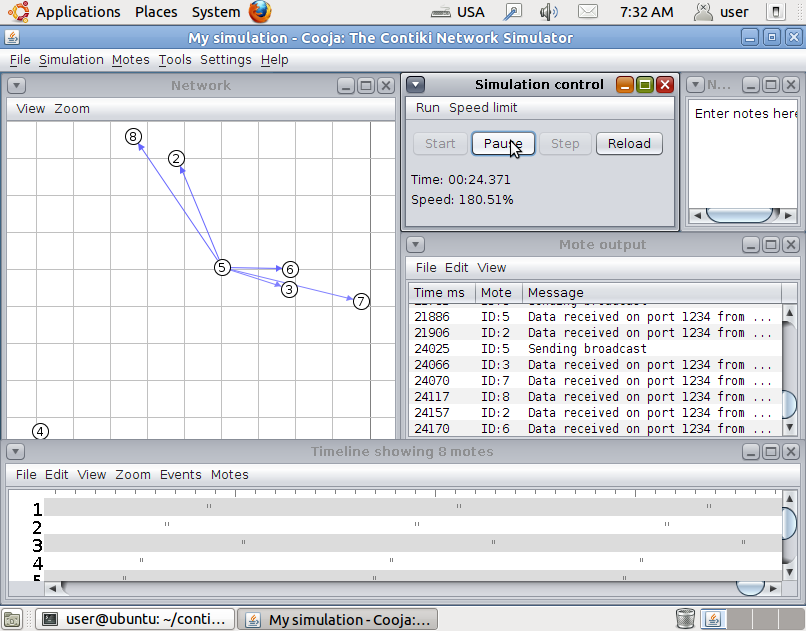
\includegraphics[width=.8\linewidth]{img/cooja.png}
	\end{figure}

\end{block}

\end{frame}

\begin{frame}

\begin{block}{Cooja -- Contiki}

	\begin{itemize}
        \item \href{https://bps90.github.io/papers/Internet-das-coisas-da-teroria-a-pratica/}{\textcolor{red}{\textbf{Minicurso - SBCR 2016}}}
        \item \href{https://www.youtube.com/watch?v=62dzCelBwIk}{\textcolor{red}{\textbf{Hands-on}}}
    \end{itemize}

\end{block}

\begin{block}{Cooja -- Contiki}

	\begin{figure}[t]
		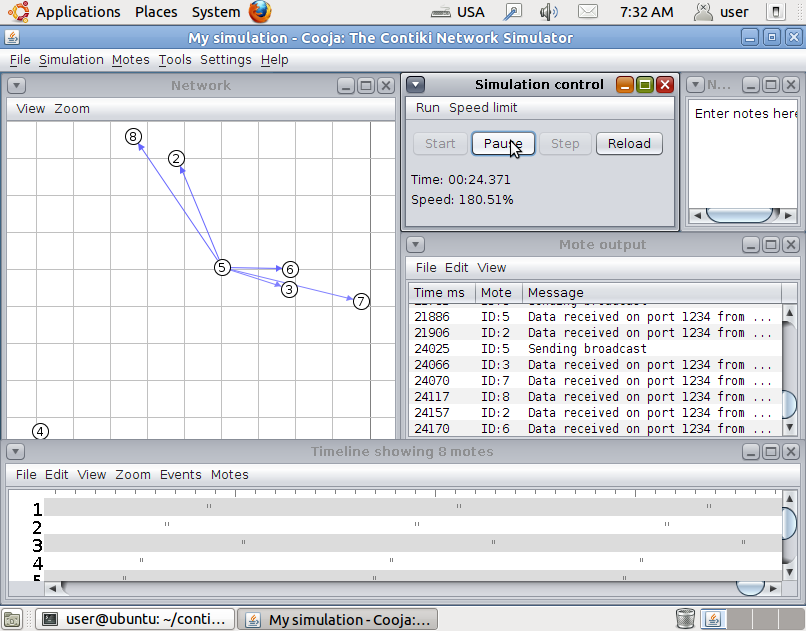
\includegraphics[width=.8\linewidth]{img/cooja.png}
	\end{figure}

\end{block}

\end{frame}
%
%------------------------------------------------
\section{Dúvidas sobre o projeto}

\subsection{Árvore de Roteamento} % Sections can be created in order to organize your presentation into discrete blocks, all sections and subsections are automatically printed in the table of contents as an overview of the talk
%------------------------------------------------
\begin{frame}
	\frametitle{Tarefa 2}
	\small
	\begin{alertblock}{Árvore para coleta de dados}
		\begin{enumerate}
			\item Faça uma inundação para descobrir o menor caminho (em saltos) de cada nó para uma Estação Base (EB).
			\item A EB deve ser iniciada através de \textbf{@NodePopupMethod}
			\item As mensagens podem ser do tipo rota ou dados
			\item O nó deve identificar se a mensagem é de construção de rota ou de dados.
			\begin{itemize}
				\item Se a mensagem é de construção de rota
				\begin{itemize}
					\item O nó deve atualizar sua rota para a EB.
				\end{itemize}
				\item Se a mensagem é de dados
				\begin{itemize}
					\item O nó deve mandar uma mensagem unicast para o próximo salto até a EB, caso exista uma rota válida
				\end{itemize}
			\end{itemize}

		\end{enumerate}
	\end{alertblock}
\end{frame}

%------------------------------------------------
\begin{frame}
	\frametitle{Tarefa 2}
	\begin{alertblock}{Árvore para coleta de dados}
		\begin{enumerate}

			\item A EB ao receber uma mensagem deve imprimir no Output informações sobre a mensagem coletada.

			\item Cada nó após ter um caminho válido para EB, deve ser permitido enviar dados periodicamente (10 rounds) para EB, isto deve ser ativado através de um \textbf{@NodePopupMethod}.

			\item O payload da mensagem de dado pode ser uma amostra de temperatura ou alguma variável de ambiente geralmente analisada por RSSF.

			\item A mensagem não pode trafegar mais que um tempo de vida estabelecido (Ex: 30 saltos)
		\end{enumerate}
	\end{alertblock}
\end{frame}

%------------------------------------------------

\begin{frame}{Dúvidas sobre o projeto.}
	\centering
	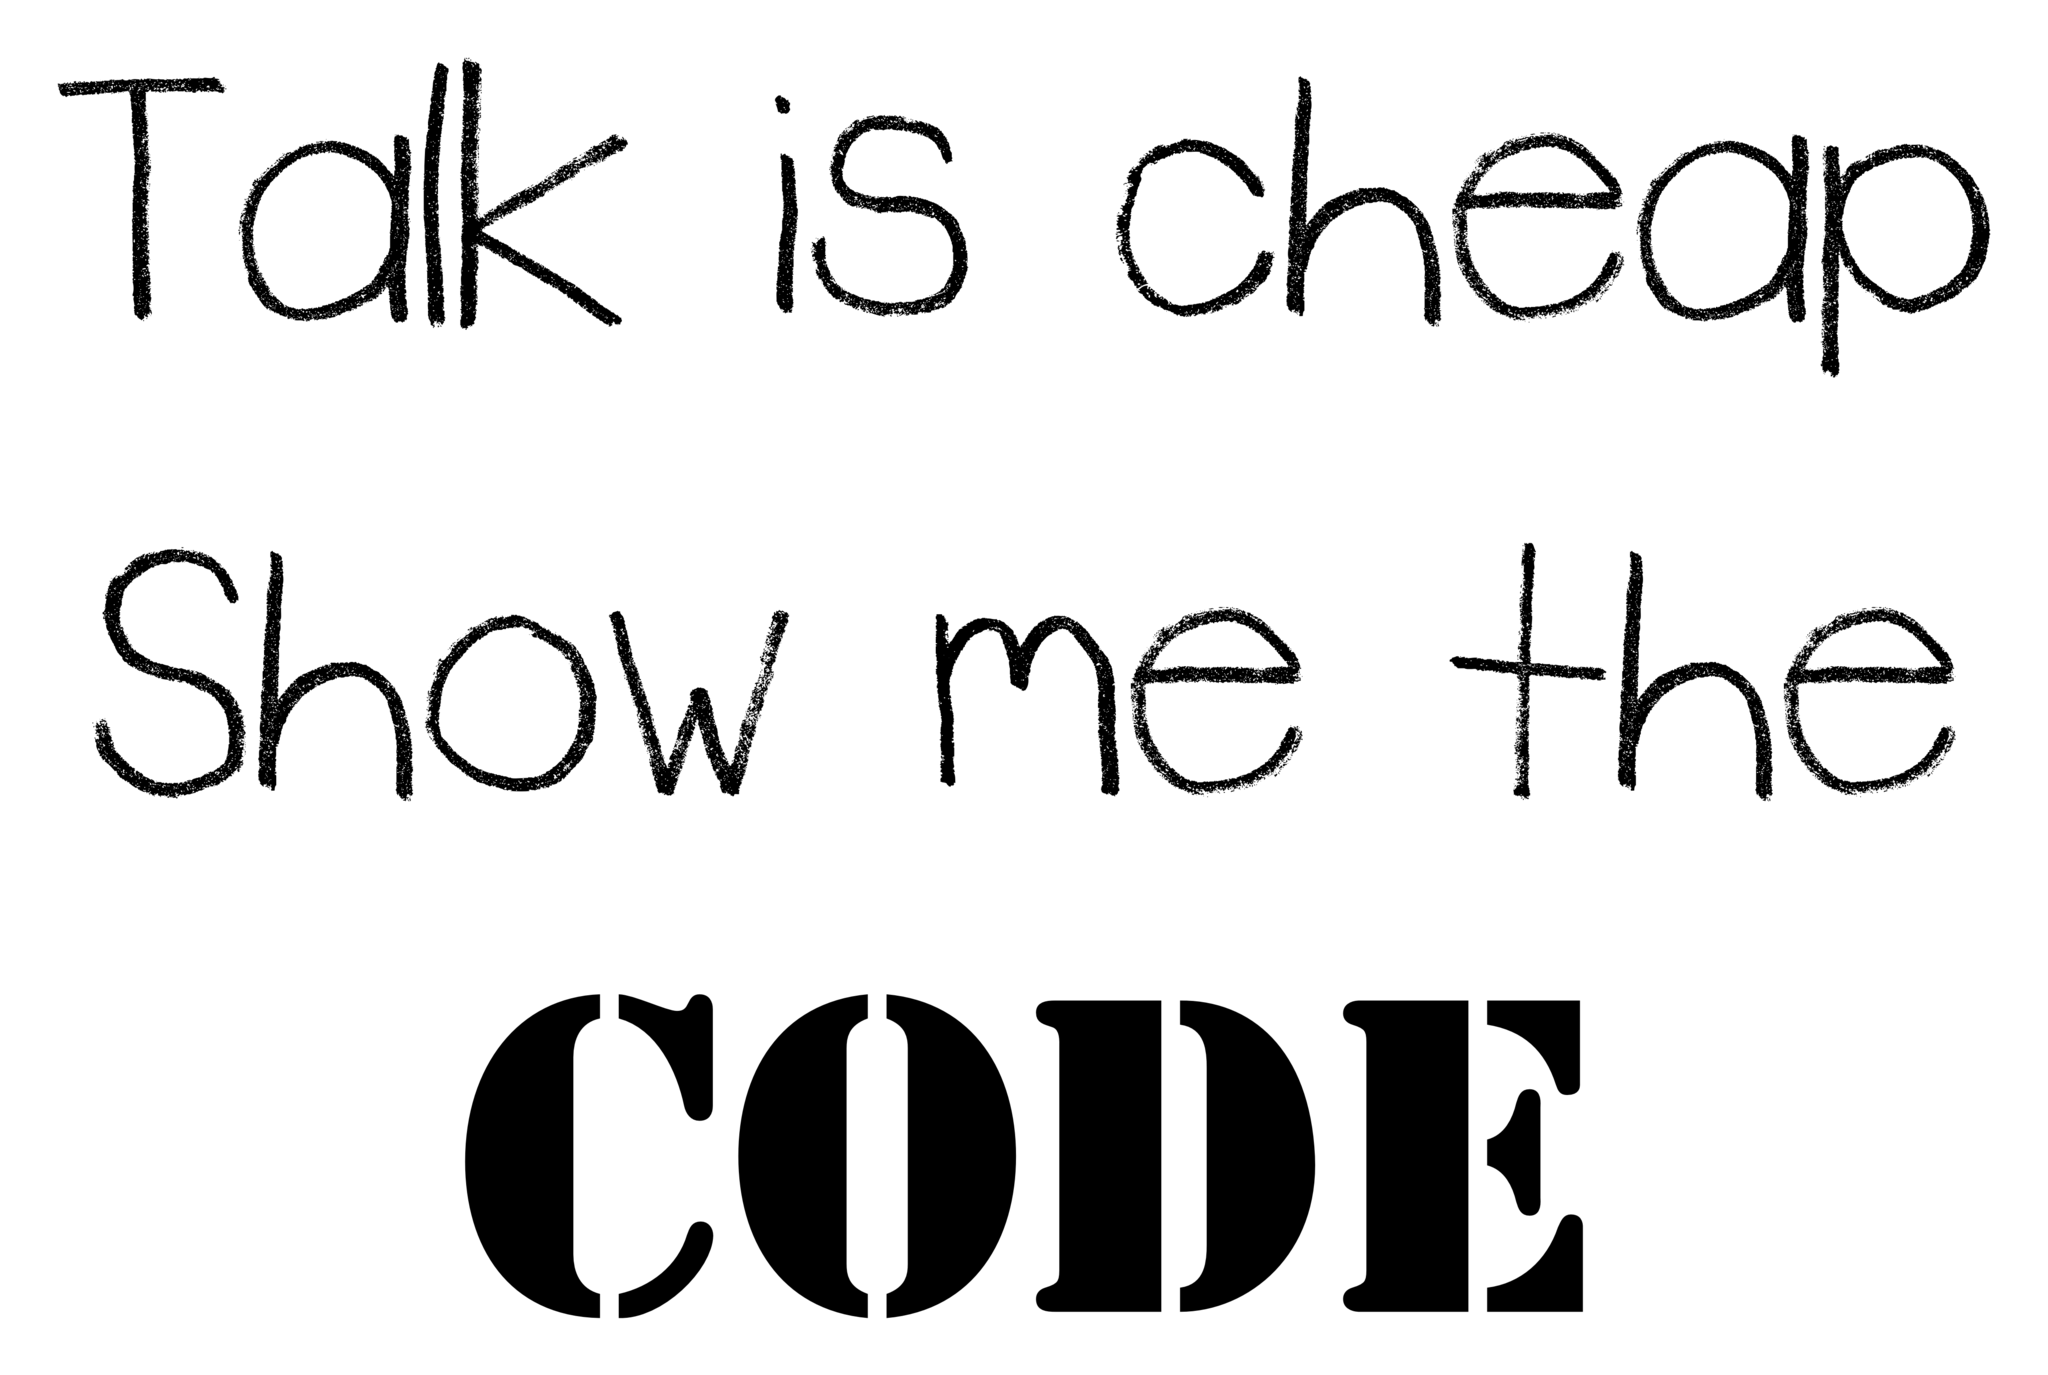
\includegraphics[width=.6\linewidth]{img/torvalds.png}
	\flushright
	--Linus
\end{frame}
%------------------------------------------------
\begin{frame}
\footnotesize
\centering

	
\includegraphics[width=0.22\linewidth]{img/git.png}
	\begin{exampleblock}{Git é vida!}
		git clone https://github.com/BrunoPereiraSantos/aula-simuladores-redes-sem-fio.git
	\end{exampleblock}

\end{frame}
\end{document}
